\section{Biological Background}

Photosystem II~\cite{oxygenicPhotosynthesis} is the protein complex responsible for the first stage of photosynthesis. Photosynthesis is a process used by plants and other organisms to convert light (photons) into energy. Photons, that are captured from the Sun or other light sources, and water are processed through a water-oxidizing enzyme known as the oxygen-evolving complex (OEC)~\cite{yano2006manganese}. The water molecule (H$_{2}$O) is split into two parts, O$_{2}$ and H$^{+}$. The O$_{2}$ is released from the system, and the H$^{+}$ will be stored and used as a source of energy.

The OEC complex performs oxidation on two water molecules through a series of intermediary states. The ``S-State Cycle''~\cite{yano2006manganese} consists of 5 states: S$_{0}$, S$_{1}$, S$_{2}$, S$_{3}$, and S$_{4}$. During the transition between each state a hydrogen electron is released. After S$_{4}$ concludes O$_{2}$ is formed. For the purpose of this work, the resting or so-called storage state S$_{1}$ will be analysed. The atomic structure of the OEC molecule is altered between each state.

The most significant feature of this compound is its inorganic core, which is \linebreak Mn$_{4}$Ca$_{1}$O$_{x}$Cl$_{1-2}$(HCO$_{3}$)$_{y}$. It is not found anywhere else in biology and is an important biological blueprint for water spliting. By studying OEC the hope is to understand how the oxidation of water can occur at such a low energy cost. Aquiring a better understanding of how the water splitting process occurs will assist in creating biomimetic catalysts or engineered PSII enzymes for real world applications. A visualization of the inorganic core of OEC in S$_{1}$ is shown in Figure~\ref{fig:oec-in-s1}~\ref{vmd}.

\begin{figure}[H]
	\centering
	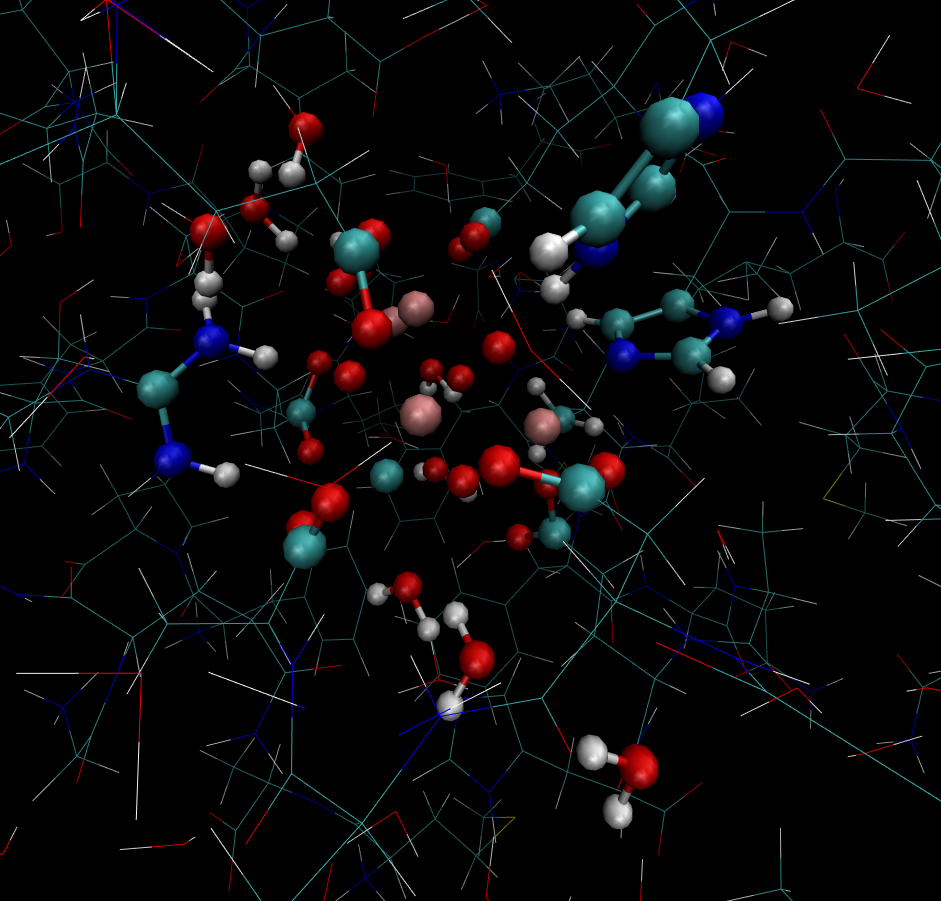
\includegraphics[bb=0 0 941 901,scale=0.3]{figures/structure.png}
	\caption{OEC Atomic Structure in S$_{1}$}
	\label{fig:oec-in-s1}
\end{figure}